\documentclass[12pt,a4paper]{ctexart}
\usepackage[margin=2.25cm]{geometry}
\usepackage{graphicx}
\usepackage{booktabs}
\usepackage{tabularx}
\usepackage{longtable}
\usepackage{array}
\usepackage{enumitem}
\usepackage{xcolor}
\usepackage{float}
\usepackage{pdflscape}
\usepackage[hidelinks]{hyperref}
\usepackage{fancyhdr}

\graphicspath{{实验2_241240041_李东泽/UML/}{实验2_241240041_李东泽/UI界面/}}
\definecolor{primary}{HTML}{5559D9}
\definecolor{soft}{HTML}{F1F2FF}
\definecolor{line}{HTML}{DDE1EC}
\definecolor{muted}{HTML}{667085}
\setlength{\parindent}{2em}
\setlength{\parskip}{0.35em}
\setlist{nosep,leftmargin=2em}
\renewcommand{\arraystretch}{1.35}
\newcolumntype{Y}{>{\raggedright\arraybackslash}X}
\newcolumntype{L}[1]{>{\raggedright\arraybackslash}p{#1}}
\pagestyle{fancy}
\fancyhf{}
\fancyhead[L]{校园二手交易系统——软件设计与建模}
\fancyhead[R]{实验二}
\fancyfoot[C]{\thepage}
\setlength{\headheight}{15pt}

\begin{document}

\begin{titlepage}
\centering
\vspace*{2.5cm}
{\Huge\bfseries 软件设计与建模实验报告\par}
\vspace{1.2cm}
{\LARGE 校园二手交易系统\par}
\vspace{0.6cm}
{\large “拾光集市”设计方案\par}
\vspace{2.3cm}
\renewcommand{\arraystretch}{1.7}
\begin{tabular}{rl}
课程实验：&实验二——软件设计与建模\\
学生姓名：&李东泽\\
学号：&241240041\\
需求来源：&实验一需求分析最终版\\
设计日期：&2026年11月6日\\
版本：&AI辅助设计初稿\\
\end{tabular}
\vfill
{\color{muted}本报告中的 UML 图均使用 PlantUML 绘制，界面原型以本地 HTML/CSS 设计稿导出。}
\end{titlepage}

\tableofcontents
\clearpage

\section{项目选择与主要功能}

\subsection{项目说明与设计范围}

本实验沿用实验一确定的“校园二手交易系统”。系统面向校园内教材、数码产品和生活用品的闲置交易，负责商品发布、审核、查询、预约和线下交易状态记录。系统不接入在线支付、退款、物流、在线聊天、竞价或第三方身份认证，也不对线下商品质量和付款结果提供担保。

系统采用响应式 Web 形态，游客可以浏览已发布商品；普通用户登录后可同时作为买家和卖家；管理员负责商品审核、举报治理、用户与分类维护、统计和日志查询。设计目标不是在实验二直接实现完整软件，而是形成边界明确、状态一致、可供后续实现的原型结构。

\subsection{主要功能模块}

\begin{longtable}{L{0.15\textwidth}L{0.19\textwidth}L{0.42\textwidth}L{0.14\textwidth}}
\toprule
模块 & 面向角色 & 主要职责 & 对应实验一需求\\
\midrule
\endfirsthead
\toprule
模块 & 面向角色 & 主要职责 & 对应实验一需求\\
\midrule
\endhead
认证与用户 & 游客、普通用户、管理员 & 注册登录、密码摘要、角色和数据归属检查、联系方式受控展示、账号禁用与恢复。 & REQ-001、013、019\\
商品与分类 & 卖家、管理员 & 草稿、商品版本、提交审核、修改、撤回、下架、分类维护和图片管理。 & REQ-002～005\\
查询与统计 & 所有角色 & 关键词、分类、价格、状态组合查询；卖家个人统计和管理员平台统计。 & REQ-006、015、018\\
审核与治理 & 管理员 & 商品审核、举报处理、违规下架、交易冻结和异常账号联动。 & REQ-003、012、013\\
预约与交易 & 买家、卖家、管理员 & 唯一预约、价格快照、卖家确认或拒绝、取消申请、超时、完成和争议处理。 & REQ-007～011、017、020\\
通知 & 普通用户 & 审核、预约、取消、超时、违规和账号状态变化的站内通知。 & REQ-014\\
日志 & 管理员、普通用户 & 追加记录关键成功、失败和冲突操作，按权限查询与导出。 & REQ-016\\
超时调度 & 系统任务 & 按服务器时间处理 24 小时未响应预约，与卖家确认进行状态竞争检查。 & REQ-010、020\\
\bottomrule
\end{longtable}

\subsection{核心数据及存储形式}

核心业务数据采用关系数据库保存。用户、商品、商品版本、审核记录、预约、取消申请、举报、争议、通知和操作日志分别建表，通过稳定编号和外键关联。MySQL 适合表达这些明确关系，也能利用事务保证商品与预约同时更新。商品图片不直接存入数据库，而是保存到对象存储，数据库只记录图片地址和顺序。

Redis 用于保存登录会话、短期幂等结果和热点查询缓存，但不作为业务最终事实来源。每次关键写操作携带请求编号；重复请求先查询幂等结果。预约创建还需要数据库层面的条件更新或唯一约束，确保同一商品同一时刻最多存在一条有效预约。即使 Redis 缓存失效，数据库约束仍能保证正确性。

\section{软件架构设计}

\subsection{架构风格与设计理由}

本系统采用“前后端分离的模块化单体”架构。前端使用 Vue 3 构建普通用户页面和管理员后台；后端使用 Spring Boot，在一个应用中按认证、商品、审核、交易、通知、统计和日志划分模块；MySQL 作为主存储，Redis 和对象存储提供辅助能力。

没有直接设计为微服务，原因有三点：第一，课程项目的规模和团队人数有限，单体应用部署、调试和测试成本更低；第二，实验一反复强调商品与预约状态一致，模块化单体可以直接使用同一数据库事务；第三，模块边界仍然明确，后续业务量增大时可以根据调用关系拆分，而不需要现在提前承担分布式事务和服务治理的复杂度。

\subsection{组件图：模块划分及交互}

\begin{figure}[H]
\centering
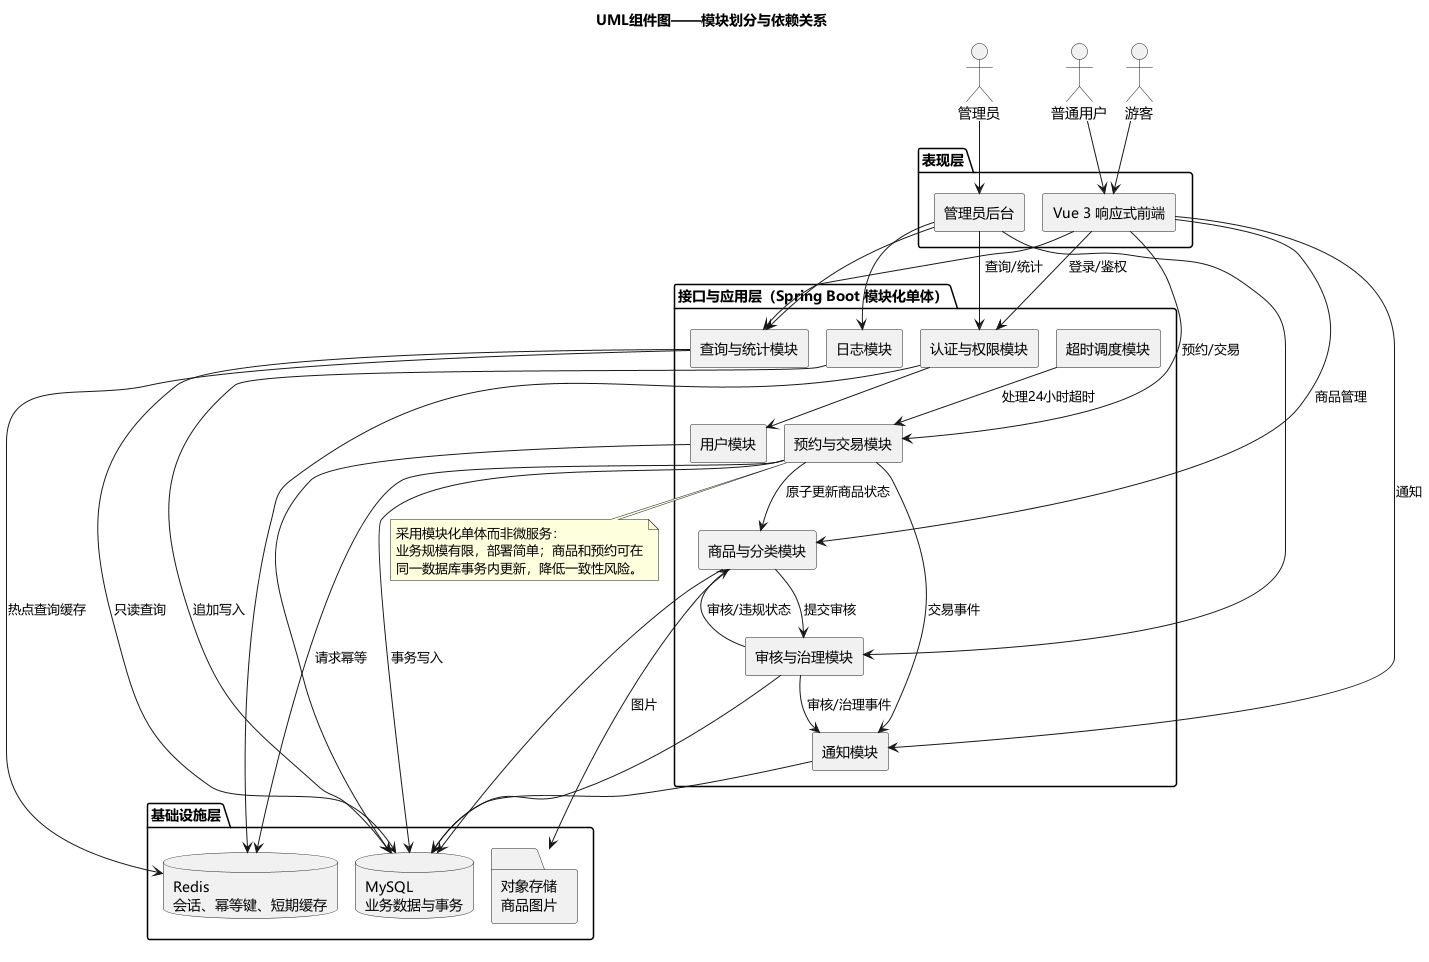
\includegraphics[width=\textwidth,height=0.76\textheight,keepaspectratio]{UML组件图.png}
\caption{UML组件图——模块划分与依赖关系}
\end{figure}

表现层只负责交互和展示，所有权限判断和状态变化在服务端完成。预约与交易模块调用商品模块完成条件状态更新，并在同一数据库事务中写入预约和日志；审核与治理模块根据处理结果更新商品或冻结交易；通知模块只消费已经确定的业务结果，避免业务失败却提前产生通知。超时调度模块调用交易模块的同一状态转换入口，不直接修改数据库。

\subsection{部署图：运行节点与技术选择}

\begin{figure}[H]
\centering
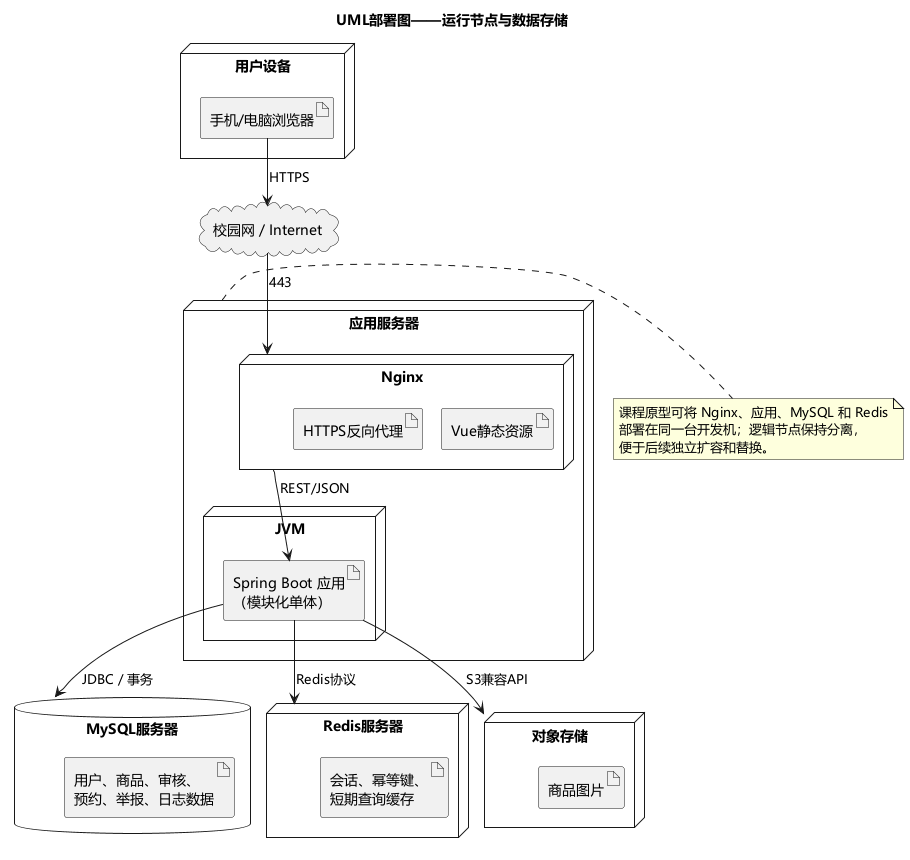
\includegraphics[height=0.72\textheight]{UML部署图.png}
\caption{UML部署图——运行节点与数据存储}
\end{figure}

课程原型可以将 Nginx、Spring Boot、MySQL 和 Redis 部署在同一台开发机，但在逻辑上仍将它们分开。浏览器只通过 HTTPS 访问 Nginx；Nginx 提供 Vue 静态资源并转发 REST 请求；应用服务器通过 JDBC 访问 MySQL，通过 Redis 协议访问缓存，通过 S3 兼容接口访问图片对象存储。该结构便于后续将数据库和对象存储迁移为独立服务。

\section{UML设计与建模}

\subsection{类图：核心领域模型}

\begin{landscape}
\begin{figure}[H]
\centering
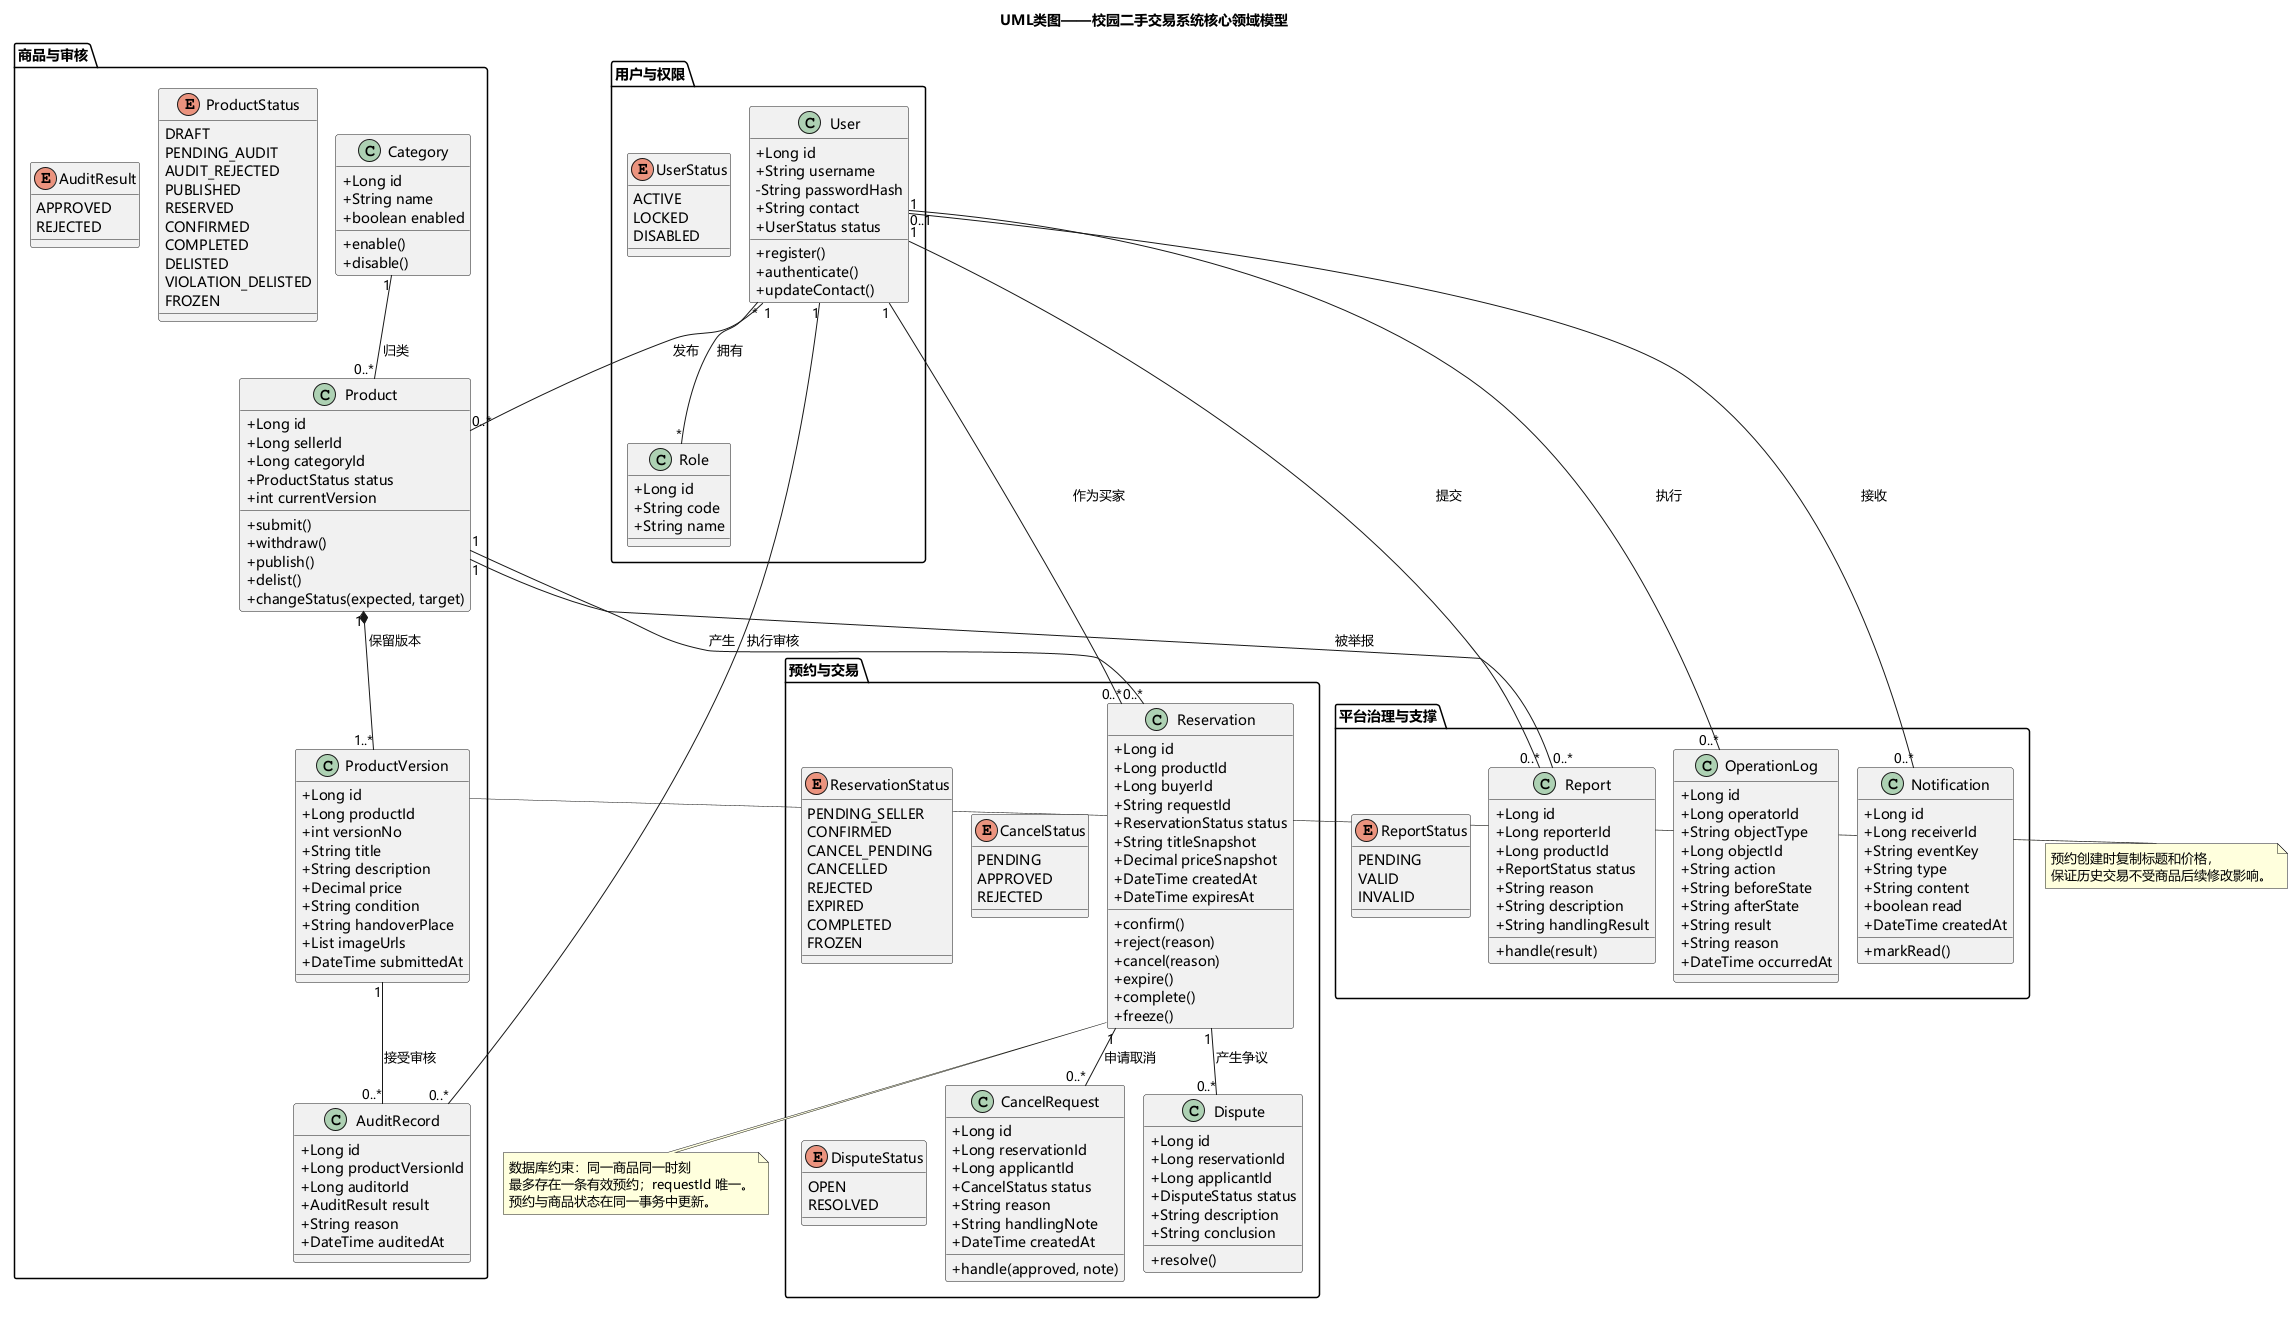
\includegraphics[width=0.96\linewidth,height=0.82\textheight,keepaspectratio]{UML类图.png}
\caption{UML类图——核心领域模型}
\end{figure}
\end{landscape}

类图没有把数据库表机械地全部画出，而是围绕领域职责组织。Product 保存商品身份和当前状态，ProductVersion 保存每次提交的可变内容，AuditRecord 指向被审核的具体版本，因此卖家再次修改不会覆盖历史依据。Reservation 在创建时复制标题和价格快照，并通过独立状态表达待确认、已确认、取消申请中、完成等过程。CancelRequest 和 Dispute 独立建模，避免把取消说明或争议结论直接塞进预约表中。

用户与角色使用多对多关系，使同一普通账号可以同时承担买家和卖家身份。操作日志只关联操作者和通用业务对象，不直接保存密码或完整联系方式。通知使用 eventKey 去重，防止请求重试或后台任务重跑造成重复提醒。

\subsection{用例图：参与者与系统边界}

\begin{figure}[H]
\centering
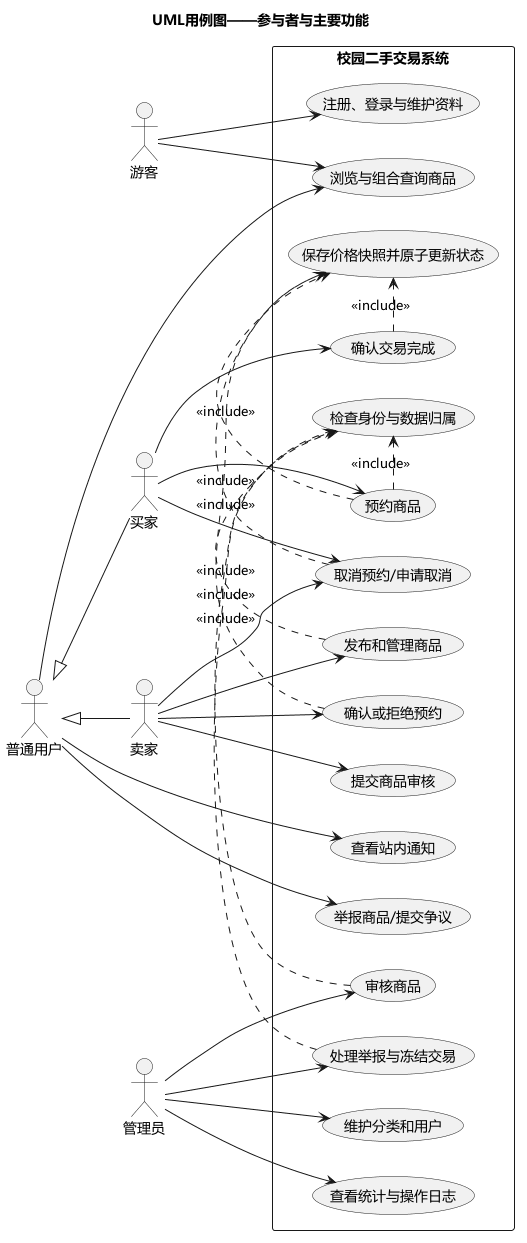
\includegraphics[height=0.78\textheight]{UML用例图.png}
\caption{UML用例图——参与者与主要功能}
\end{figure}

用例图显示游客、普通用户、买家、卖家和管理员之间的继承关系。买家和卖家都是普通用户在一次业务中的角色，不需要注册两套账号。预约、取消、处理预约和完成交易都包含“保存价格快照并原子更新状态”用例；所有写操作和管理员操作都包含身份与数据归属检查。

\subsection{状态图：商品生命周期}

\begin{figure}[H]
\centering
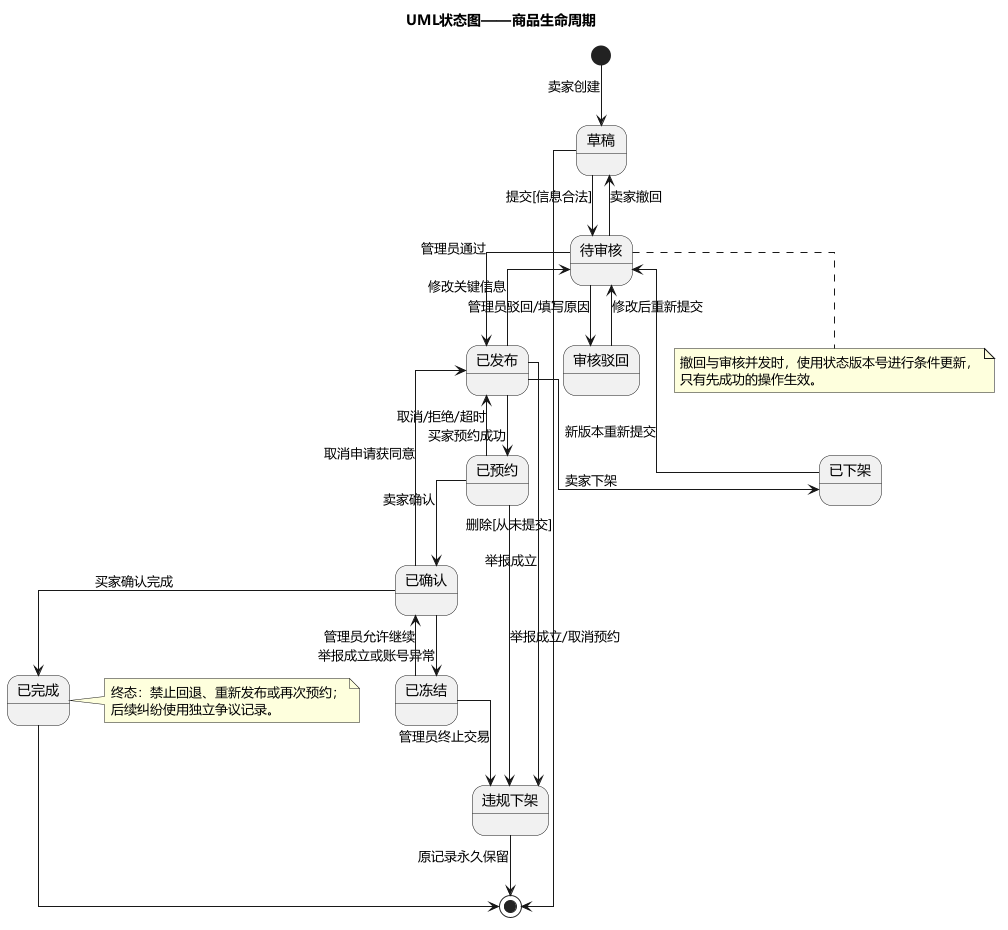
\includegraphics[height=0.76\textheight]{UML商品状态图.png}
\caption{UML状态图——商品生命周期}
\end{figure}

商品状态图以实验一确认的状态基线为准。草稿只有在信息合法时才能提交；待审核商品可以被卖家撤回，也可以被管理员通过或驳回。商品发布后，修改关键信息必须重新审核。已预约状态可以因取消、拒绝或超时恢复发布，也可以由卖家确认进入已确认。已完成是不可回退的终态；违规下架的原记录永久保留，整改只能复制为新草稿。

\subsection{活动图：预约、取消和完成流程}

\begin{figure}[H]
\centering
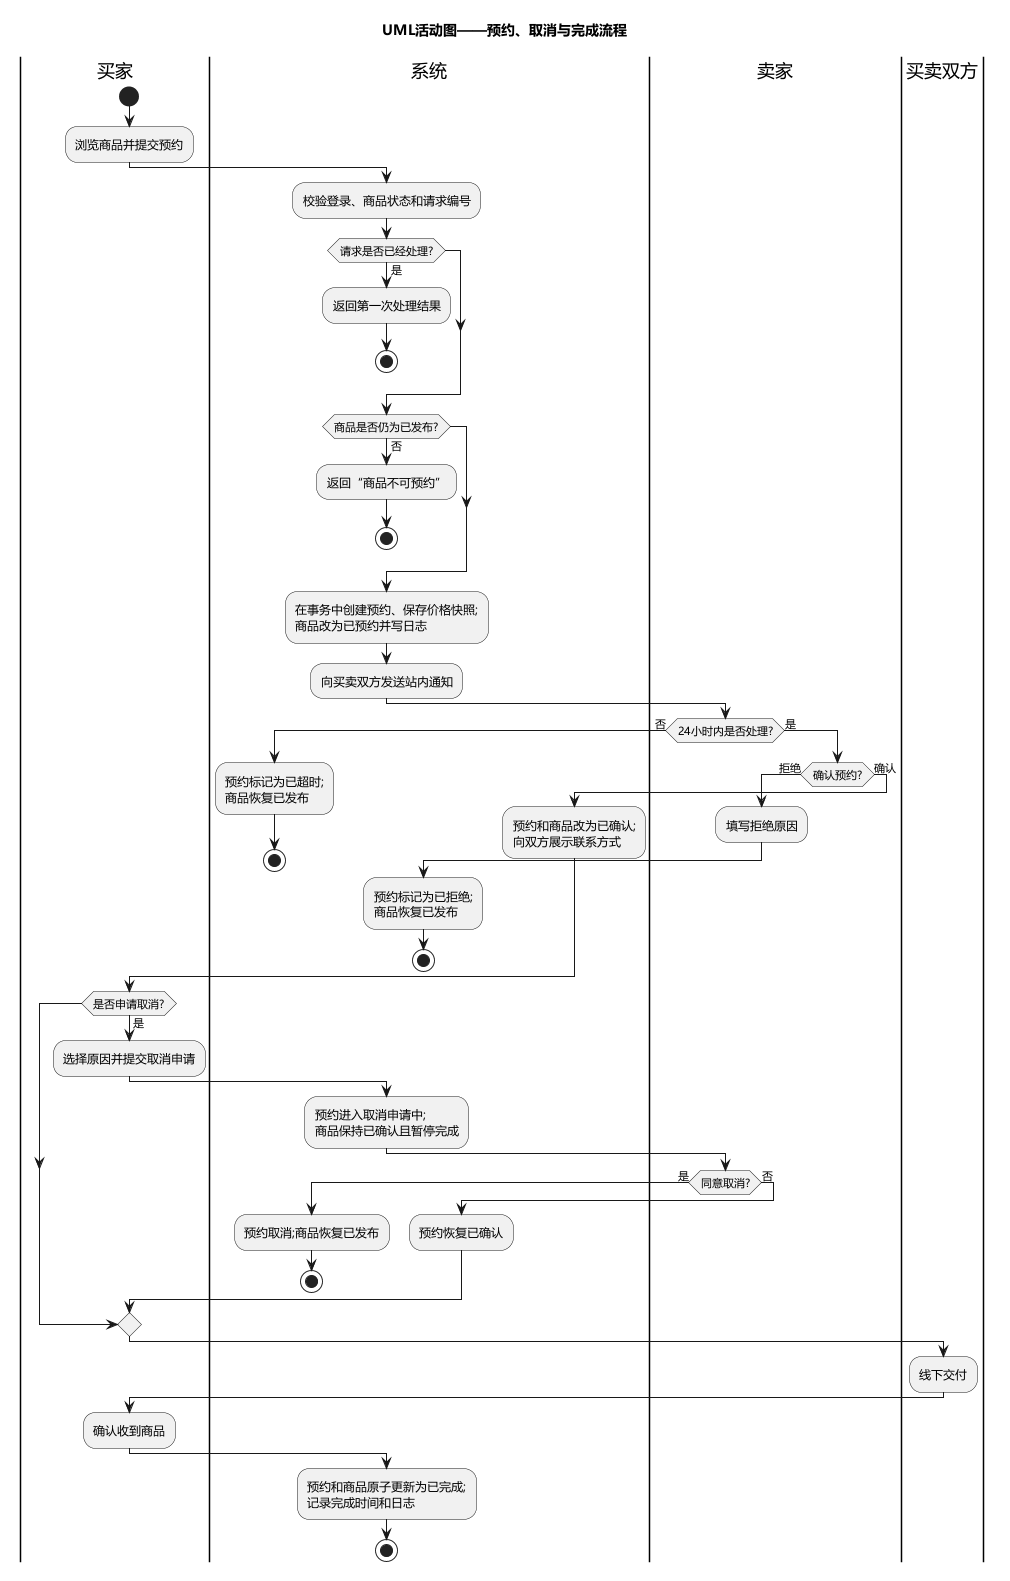
\includegraphics[height=0.81\textheight]{UML预约活动图.png}
\caption{UML活动图——预约、取消与完成流程}
\end{figure}

活动图用泳道区分买家、系统、卖家和线下交付环节。系统在预约前先检查幂等键和商品当前状态；卖家 24 小时未处理时由系统超时；卖家确认后，买家若申请取消，商品保持已确认并暂停确认完成，直到卖家处理申请。该图同时说明线下交付不由系统执行，系统只记录交付后的确认结果。

\subsection{时序图：并发预约与幂等}

\begin{landscape}
\begin{figure}[H]
\centering
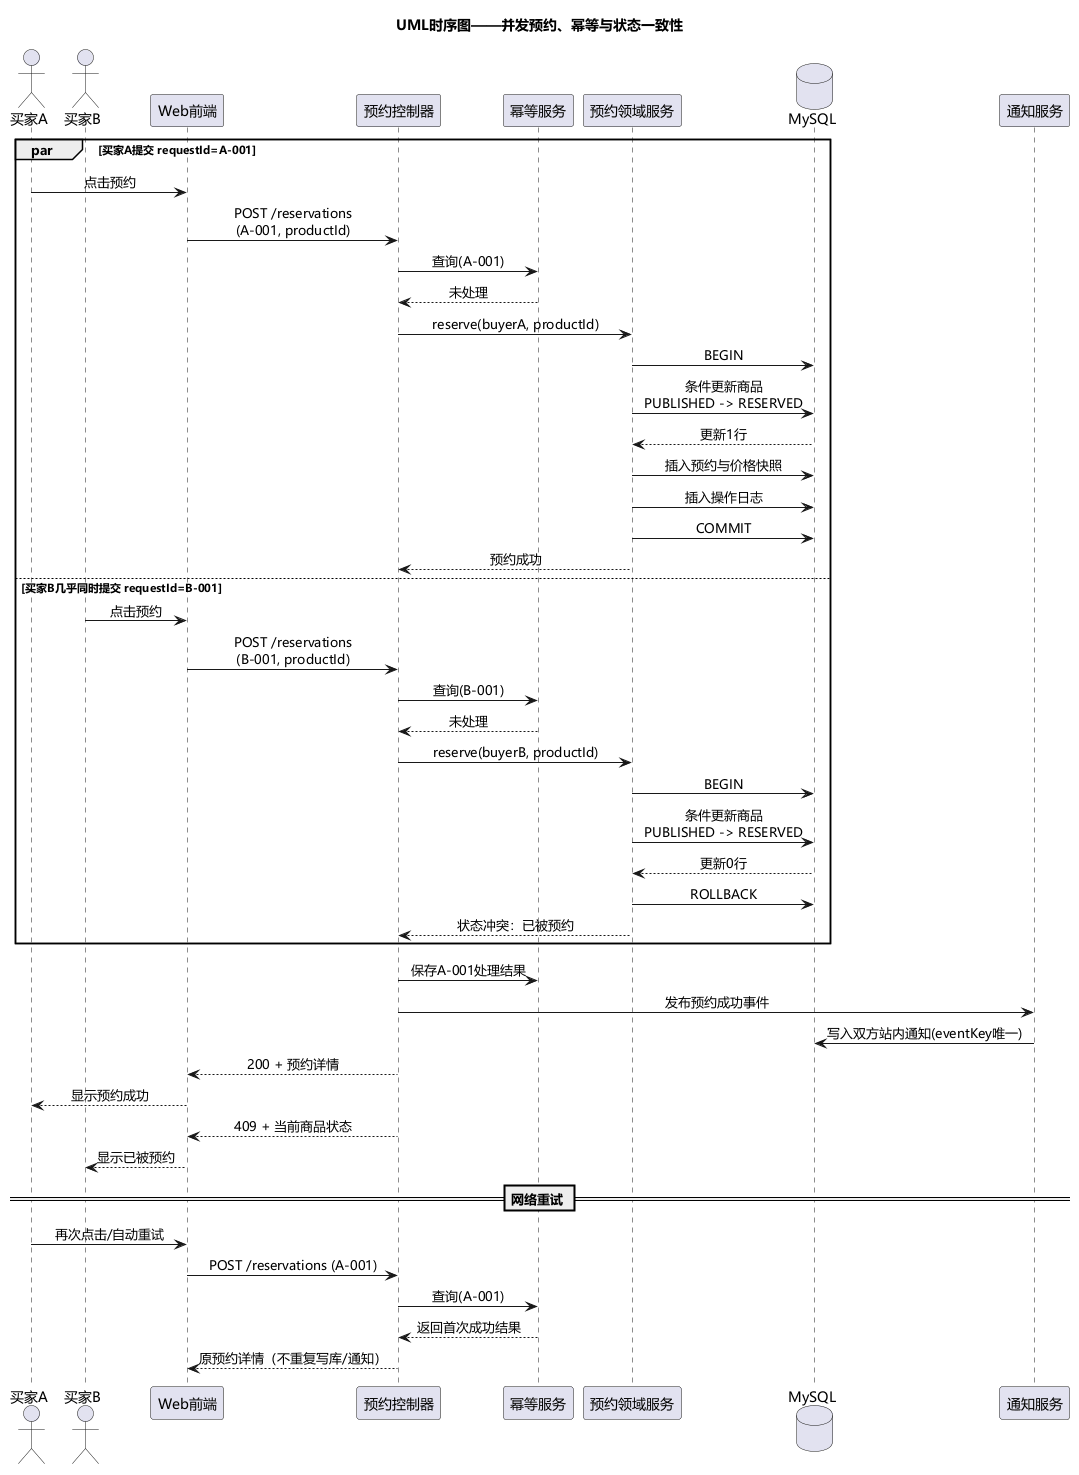
\includegraphics[width=0.94\linewidth,height=0.82\textheight,keepaspectratio]{UML预约交易时序图.png}
\caption{UML时序图——并发预约、幂等与状态一致性}
\end{figure}
\end{landscape}

两个买家几乎同时预约时，预约服务使用“当前状态必须为 PUBLISHED”的条件更新。买家 A 更新一行并在同一事务中写入预约、价格快照和日志；买家 B 更新零行，事务回滚并获得状态冲突结果。A 的网络重试沿用原 requestId，幂等服务直接返回第一次结果，不重复写库和通知。该设计同时应对多人争抢、重复点击和旧页面操作。

\section{UI界面设计}

\subsection{视觉规范和交互原则}

原型名称为“拾光集市”。主色使用蓝紫色，表达校园、可信和年轻感；成功、待处理、冲突分别使用绿色、橙色和红色，且状态不仅依靠颜色，还保留文字标签。普通用户和管理员共享相同的字号、卡片、按钮和状态组件，但使用不同导航结构。所有会改变状态的危险操作均提供明确按钮、原因输入或二次确认。

页面遵循三项原则：第一，状态优先，商品与预约的当前状态应在页面首屏可见；第二，权限可见，用户只看到当前角色能够执行的操作；第三，异常可解释，超时、驳回、冲突和取消不只提示失败，还显示原因和下一步。

\subsection{游客与账户模块}

\begin{figure}[H]
\centering
\begin{minipage}[t]{0.49\textwidth}\centering
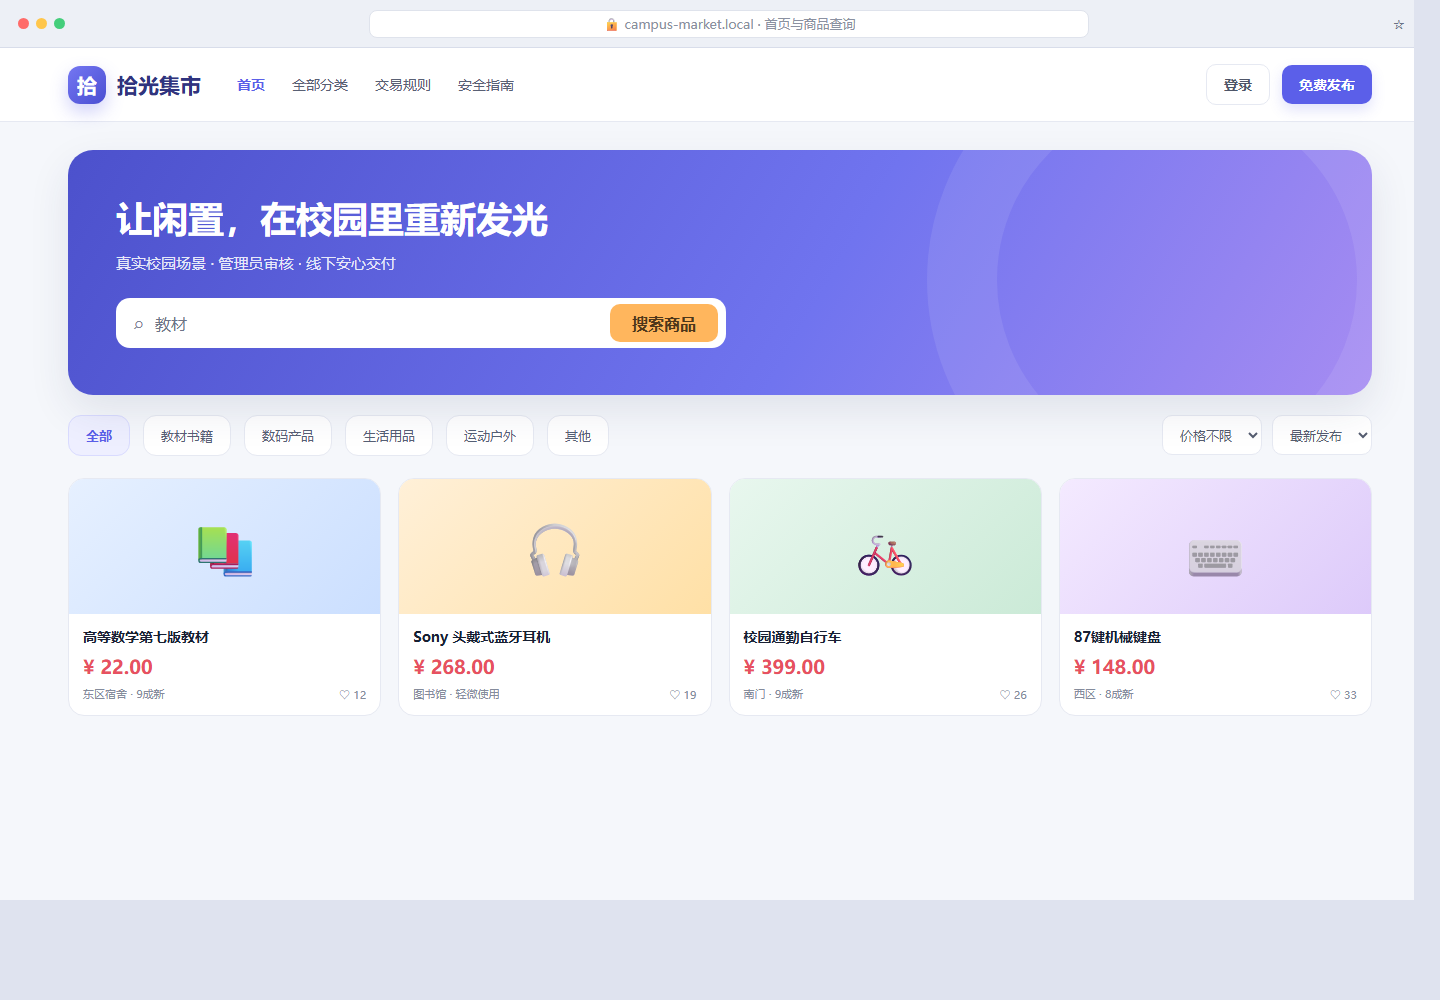
\includegraphics[width=\linewidth]{01_首页与商品查询.png}
\caption*{UI-01：首页与商品查询}
\end{minipage}\hfill
\begin{minipage}[t]{0.49\textwidth}\centering
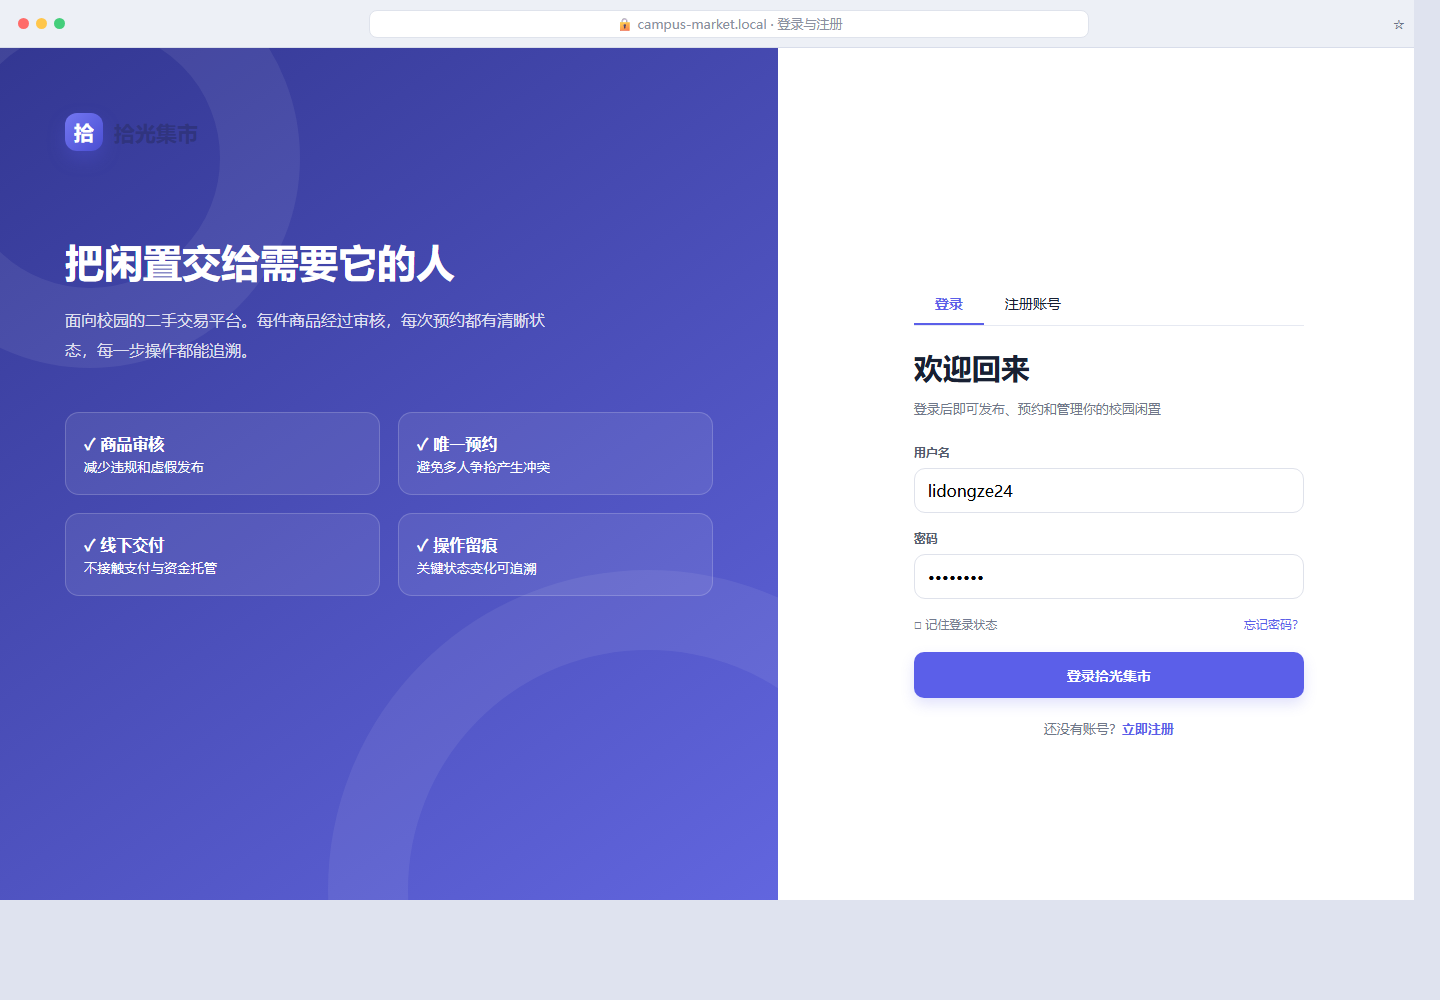
\includegraphics[width=\linewidth]{02_登录与注册.png}
\caption*{UI-02：登录与注册}
\end{minipage}
\caption{游客浏览与账户入口}
\end{figure}

首页将关键词搜索、分类、价格和排序集中在商品列表之前，游客无需登录即可使用。登录页在表单旁说明商品审核、唯一预约、线下交付和操作留痕，让用户在进入系统前理解业务边界。注册与登录共用同一入口，管理员账号不在公开页面注册。

\subsection{商品浏览与卖家管理模块}

\begin{figure}[H]
\centering
\begin{minipage}[t]{0.49\textwidth}\centering
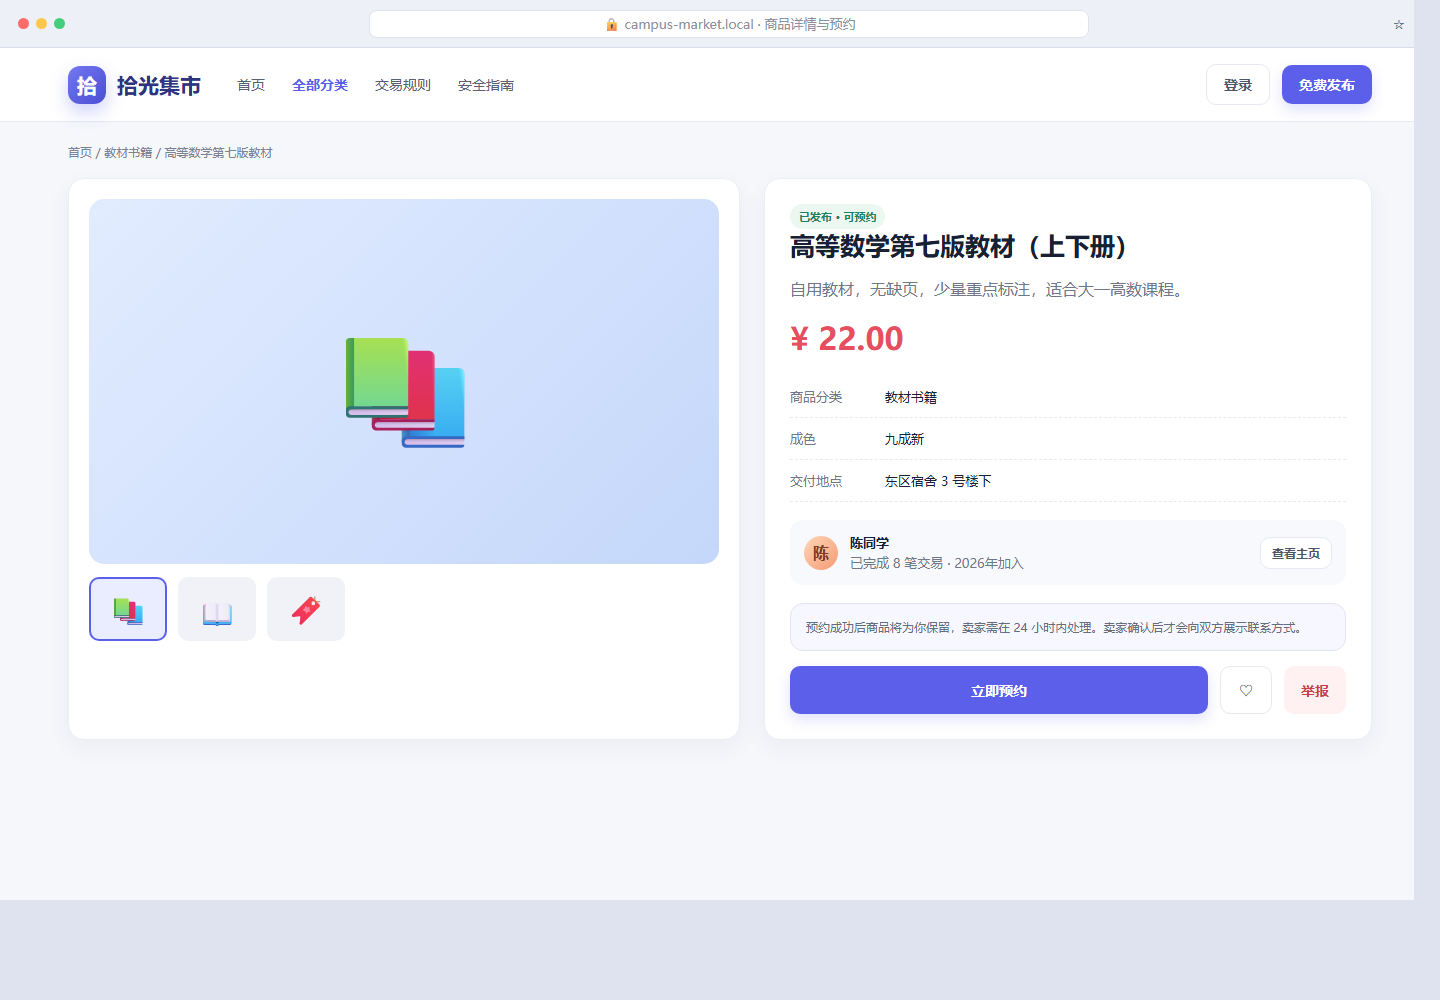
\includegraphics[width=\linewidth]{03_商品详情与预约.png}
\caption*{UI-03：商品详情与预约}
\end{minipage}\hfill
\begin{minipage}[t]{0.49\textwidth}\centering
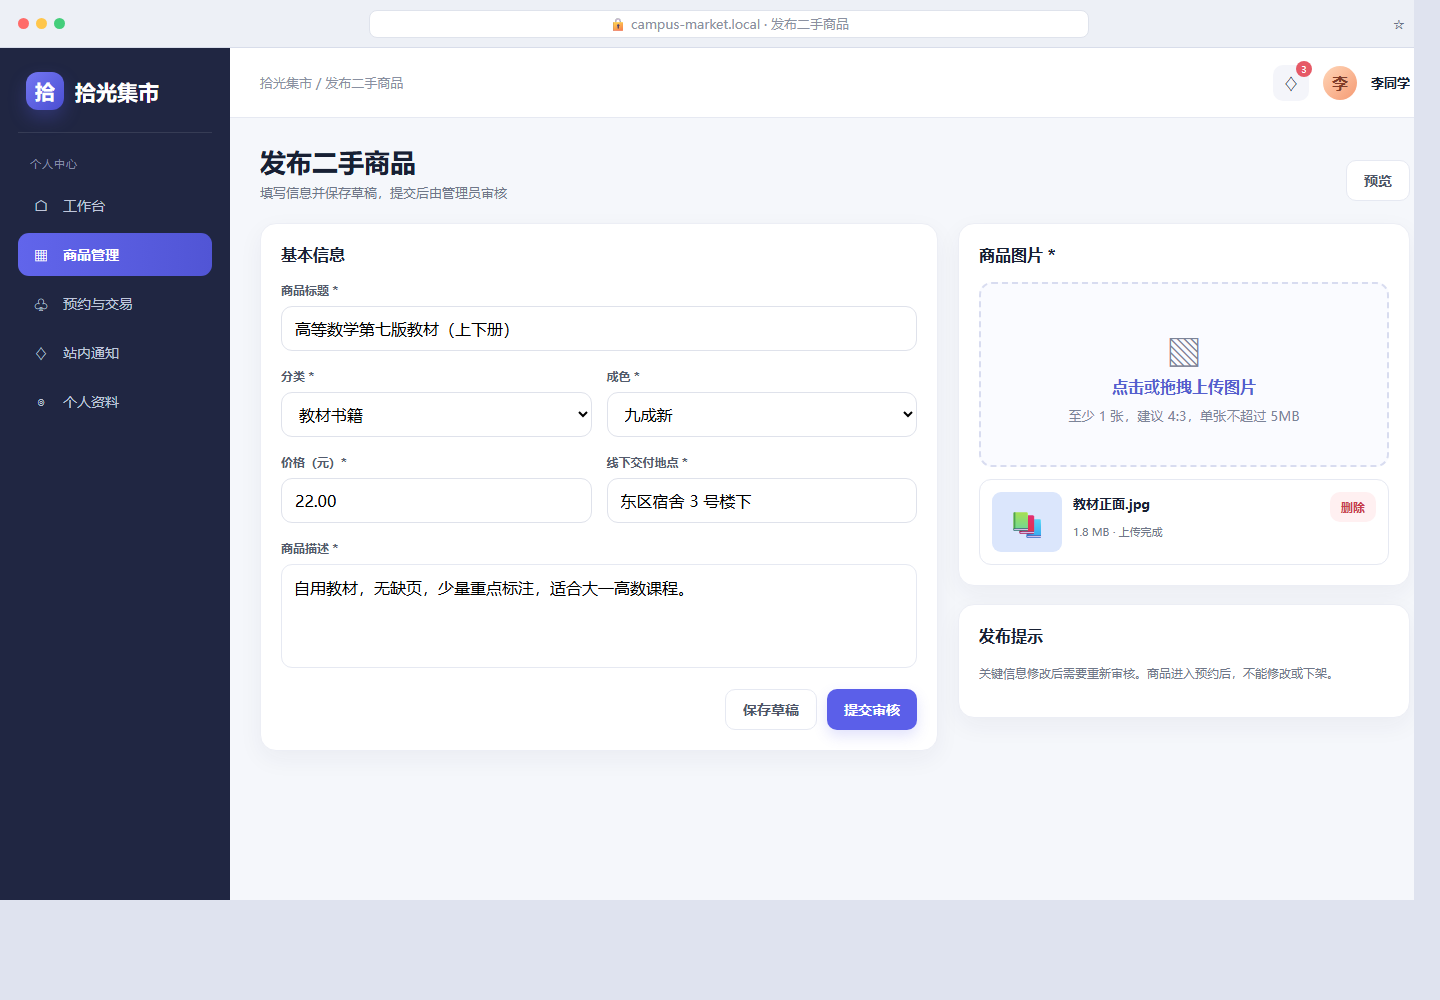
\includegraphics[width=\linewidth]{04_发布编辑商品.png}
\caption*{UI-04：发布和编辑商品}
\end{minipage}
\caption{商品查看与信息录入}
\end{figure}

商品详情页展示当前是否可预约、价格、成色、交付地点、卖家概况和预约规则，联系方式在确认前不展示。发布页按基本信息和图片拆分，价格、分类和必填项具有明确输入位置，并提示“关键信息修改后重新审核”。

\begin{figure}[H]
\centering
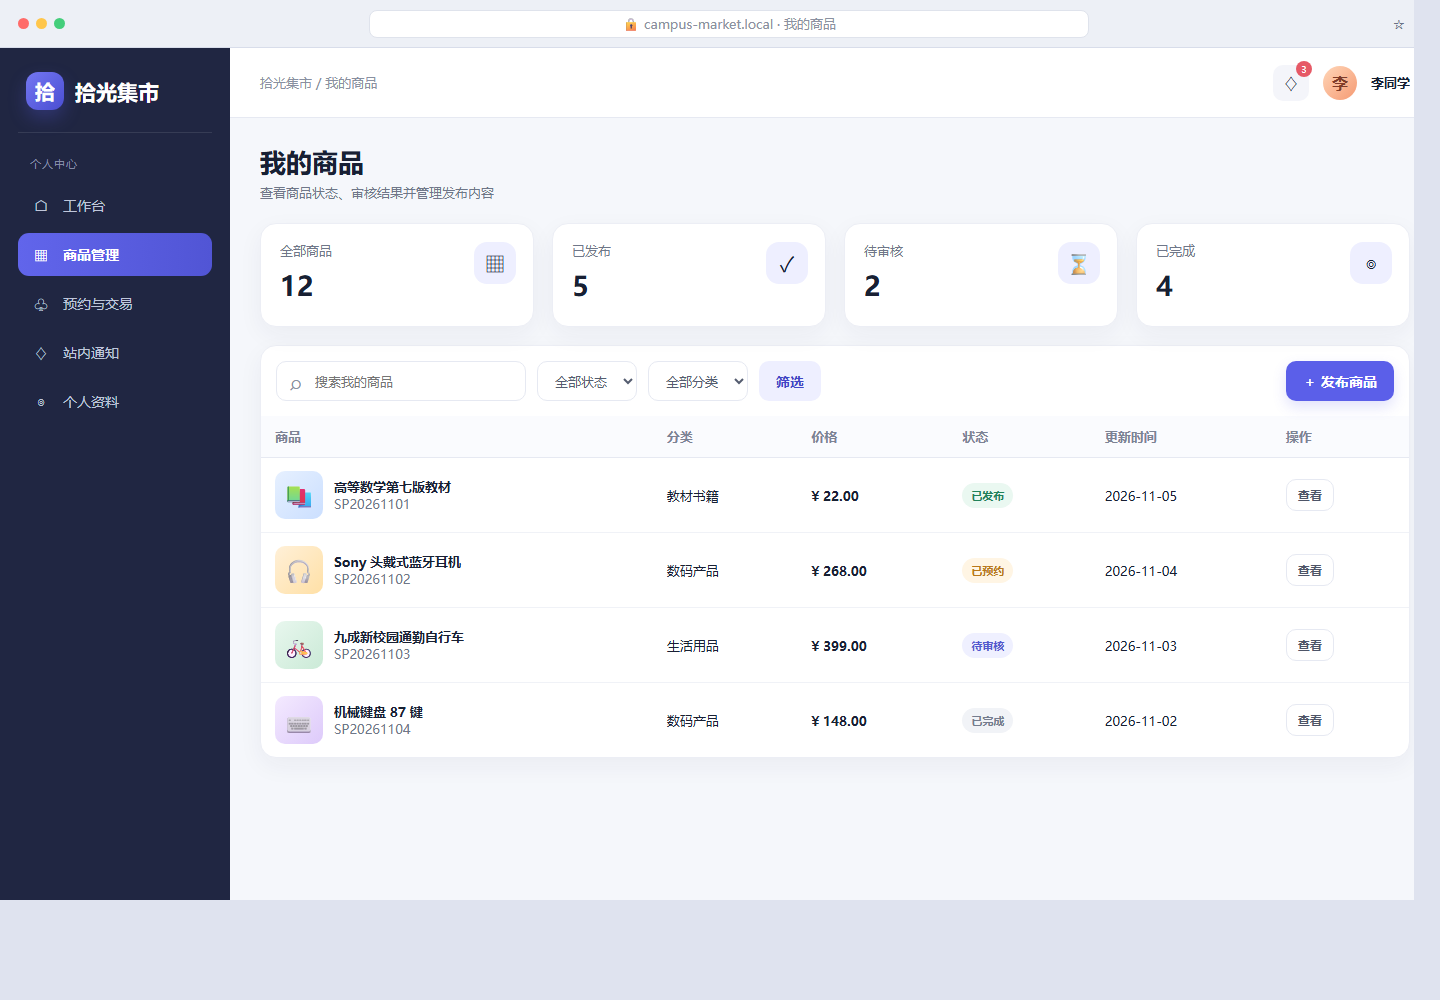
\includegraphics[width=0.82\textwidth]{05_卖家商品管理.png}
\caption{UI-05：卖家商品管理}
\end{figure}

卖家商品管理页用统计卡片和状态表格展示草稿、待审核、已发布、已预约和已完成商品。按钮根据状态出现，例如已预约商品不会显示编辑或直接下架，以界面限制配合服务端状态检查。

\subsection{预约、交易与通知模块}

\begin{figure}[H]
\centering
\begin{minipage}[t]{0.49\textwidth}\centering
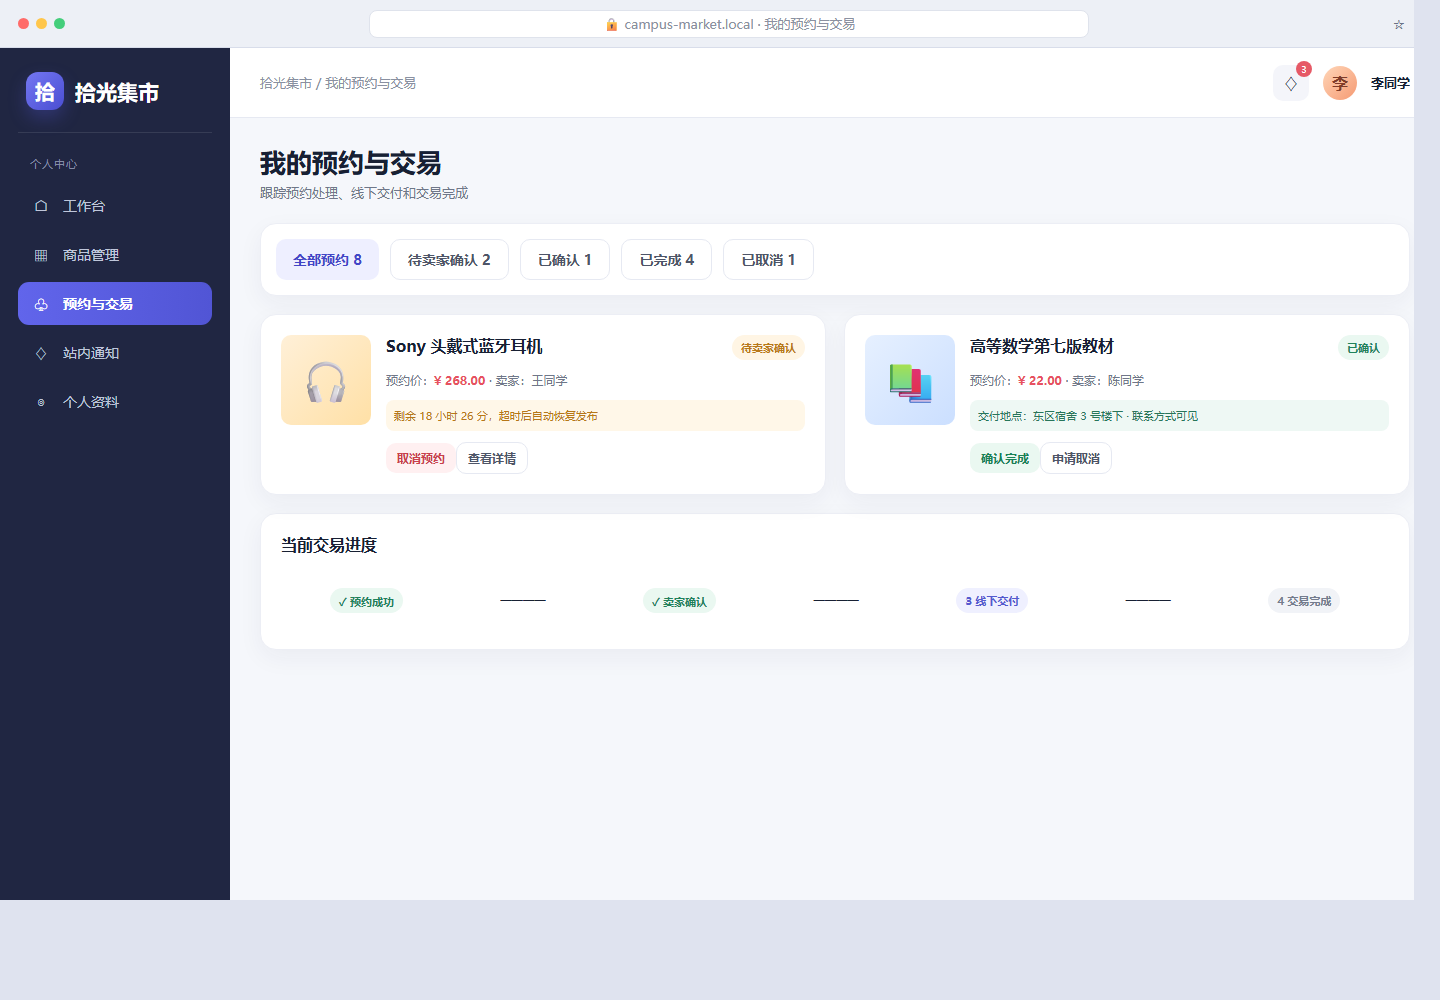
\includegraphics[width=\linewidth]{06_我的预约与交易.png}
\caption*{UI-06：我的预约与交易}
\end{minipage}\hfill
\begin{minipage}[t]{0.49\textwidth}\centering
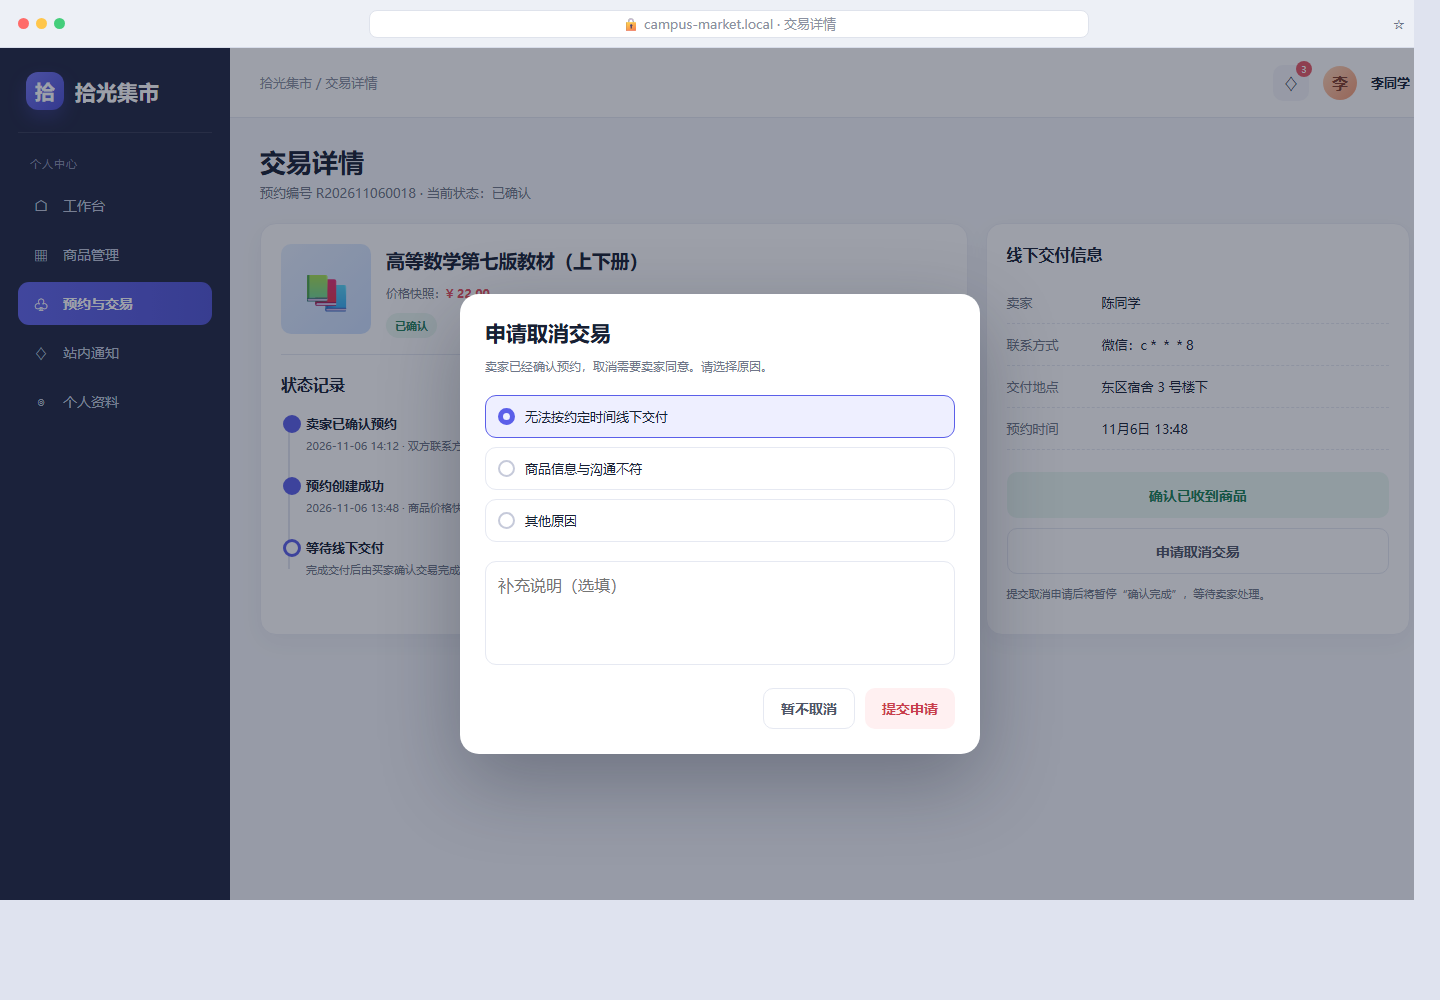
\includegraphics[width=\linewidth]{07_取消申请与交易详情.png}
\caption*{UI-07：取消申请与交易详情}
\end{minipage}
\caption{预约状态和取消交互}
\end{figure}

预约列表突出 24 小时剩余时间、是否已经确认、交付地点和下一步操作。交易确认后，取消不再是直接按钮，而是申请流程；弹窗要求选择原因，并明确告知需要卖家同意。取消申请提交后，“确认完成”暂停，避免两个互斥操作同时发生。

\begin{figure}[H]
\centering
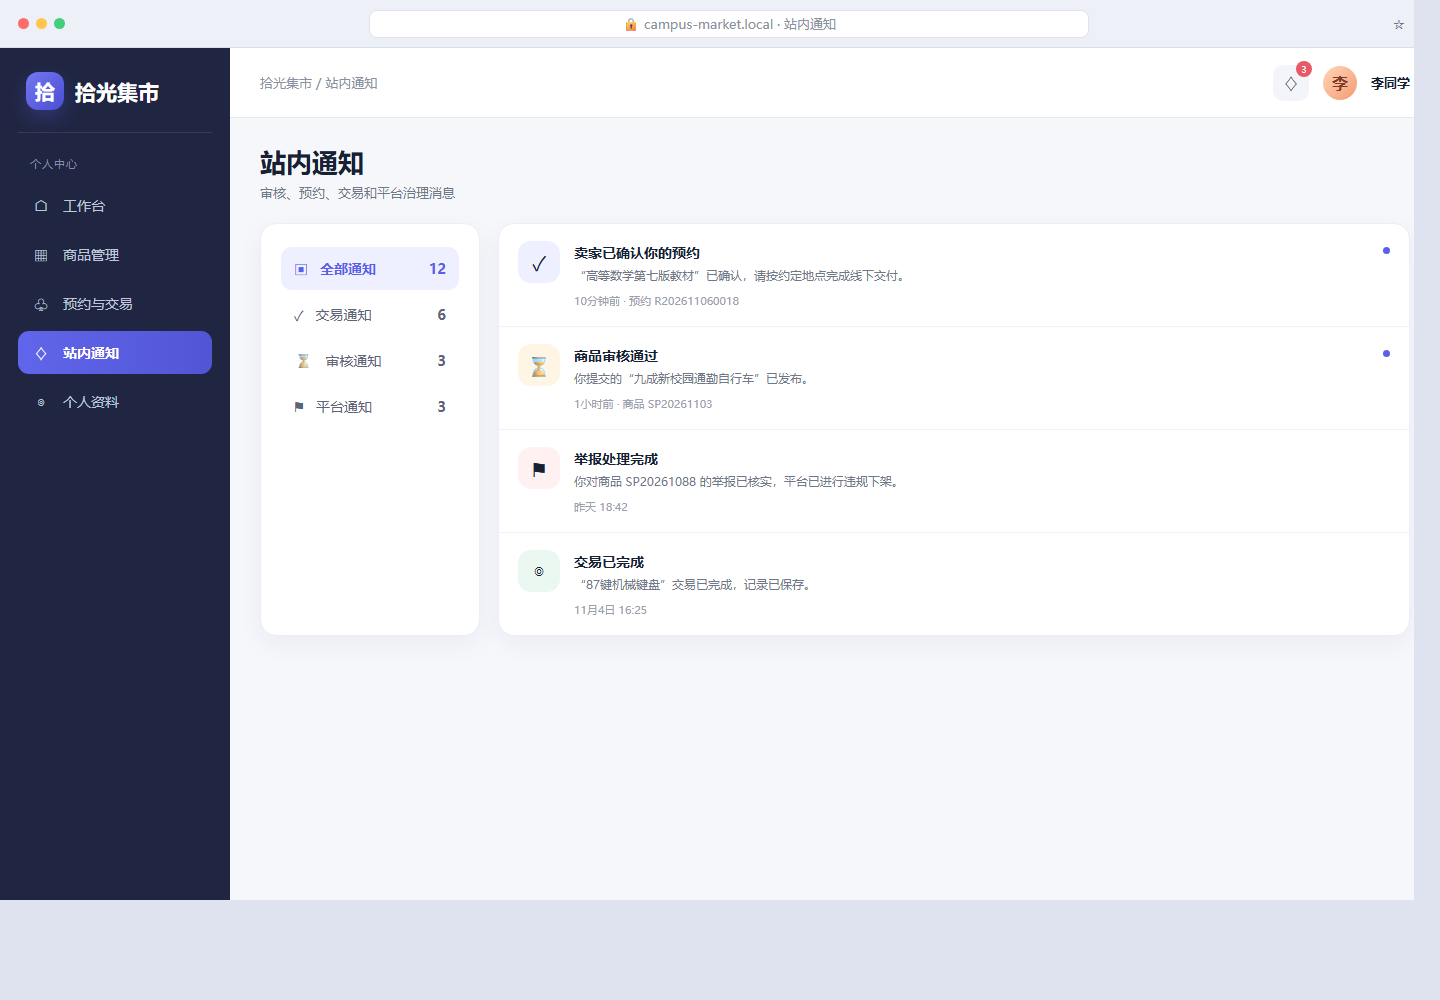
\includegraphics[width=0.82\textwidth]{08_站内通知.png}
\caption{UI-08：站内通知}
\end{figure}

通知按交易、审核和平台消息分类，每条通知显示关联对象和发生时间。eventKey 用于后端去重；前端未读圆点只表示阅读状态，不影响业务结果。

\subsection{管理员后台模块}

\begin{figure}[H]
\centering
\begin{minipage}[t]{0.49\textwidth}\centering
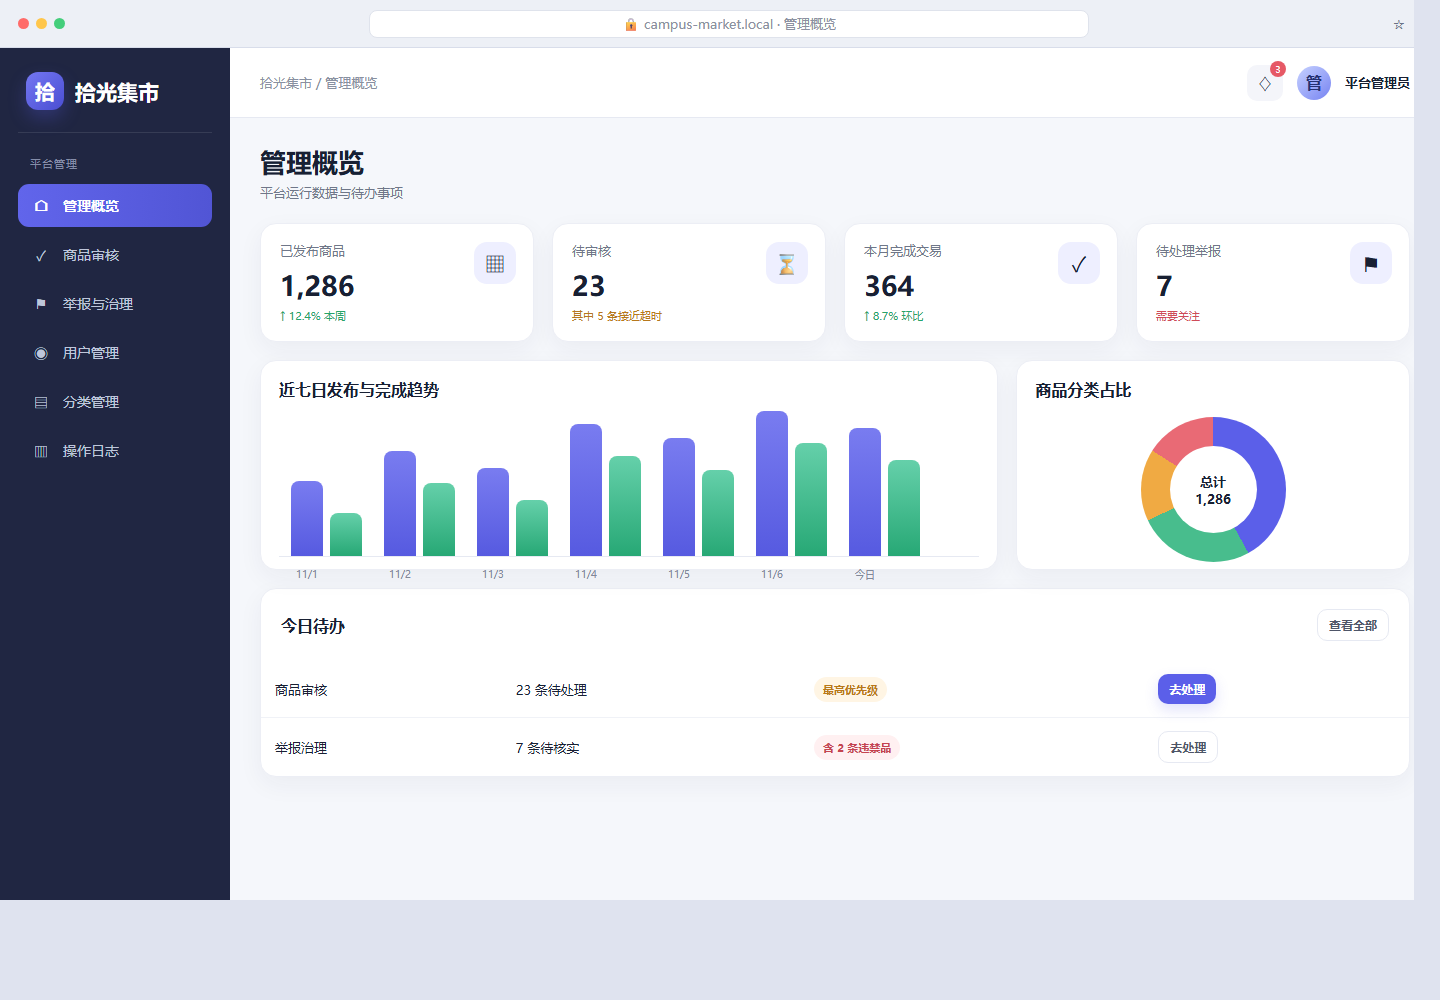
\includegraphics[width=\linewidth]{09_管理员仪表盘.png}
\caption*{UI-09：管理员仪表盘}
\end{minipage}\hfill
\begin{minipage}[t]{0.49\textwidth}\centering
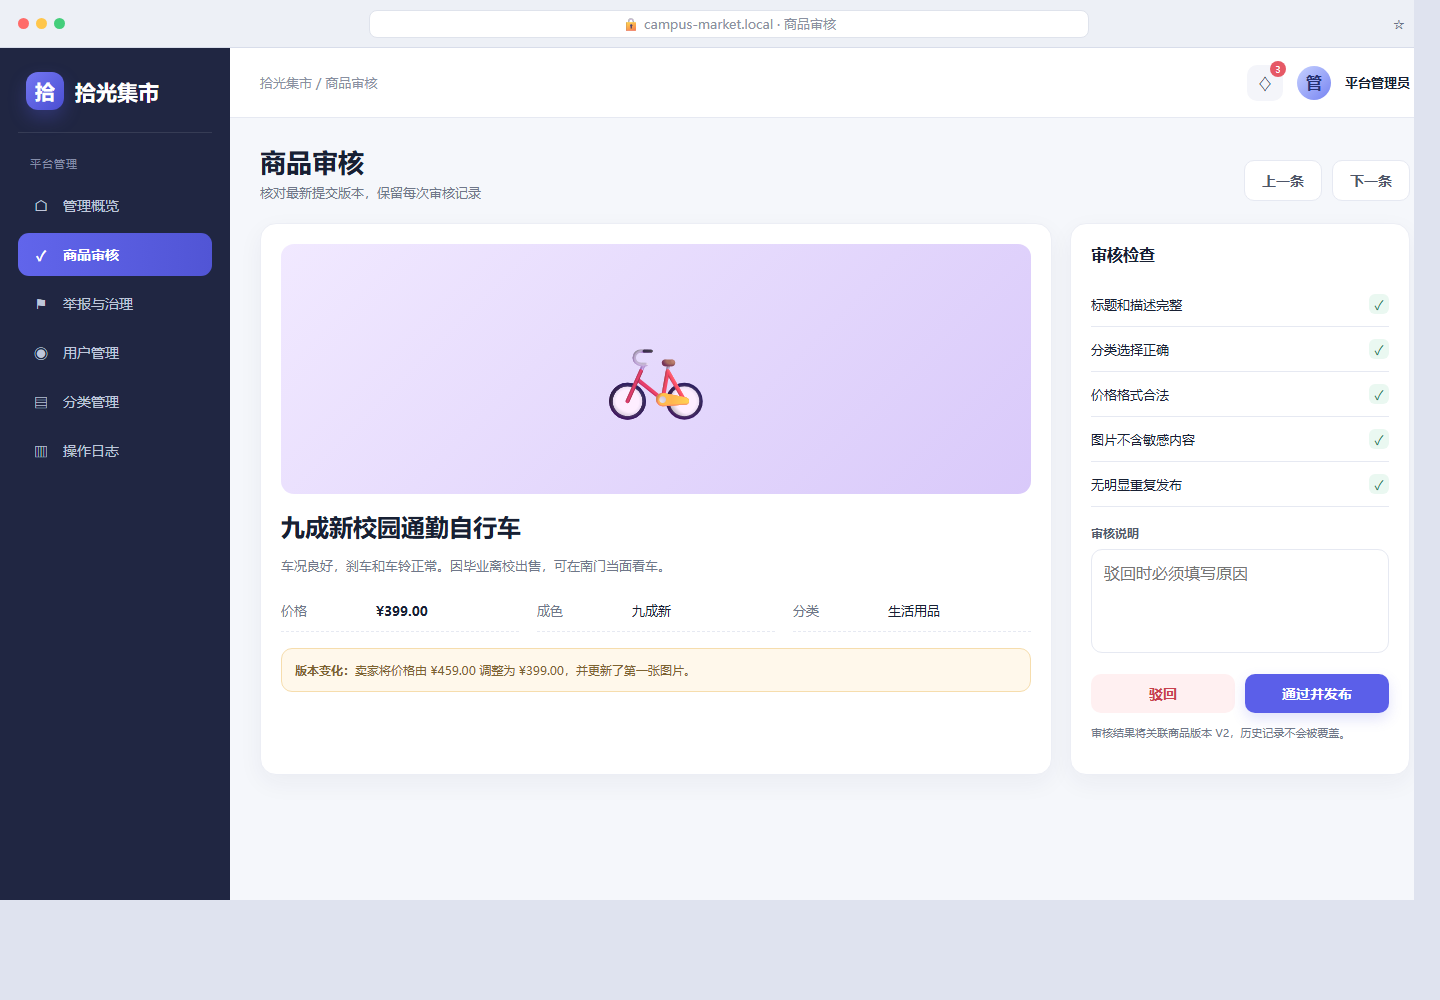
\includegraphics[width=\linewidth]{10_商品审核.png}
\caption*{UI-10：商品审核}
\end{minipage}
\caption{平台概览与商品审核}
\end{figure}

管理概览突出待审核和待处理举报，不只展示累计数字。审核页显示商品当前提交版本和与上一版本的变化；通过与驳回分别使用主按钮和危险按钮，驳回时必须填写原因，处理结果关联具体版本。

\begin{figure}[H]
\centering
\begin{minipage}[t]{0.49\textwidth}\centering
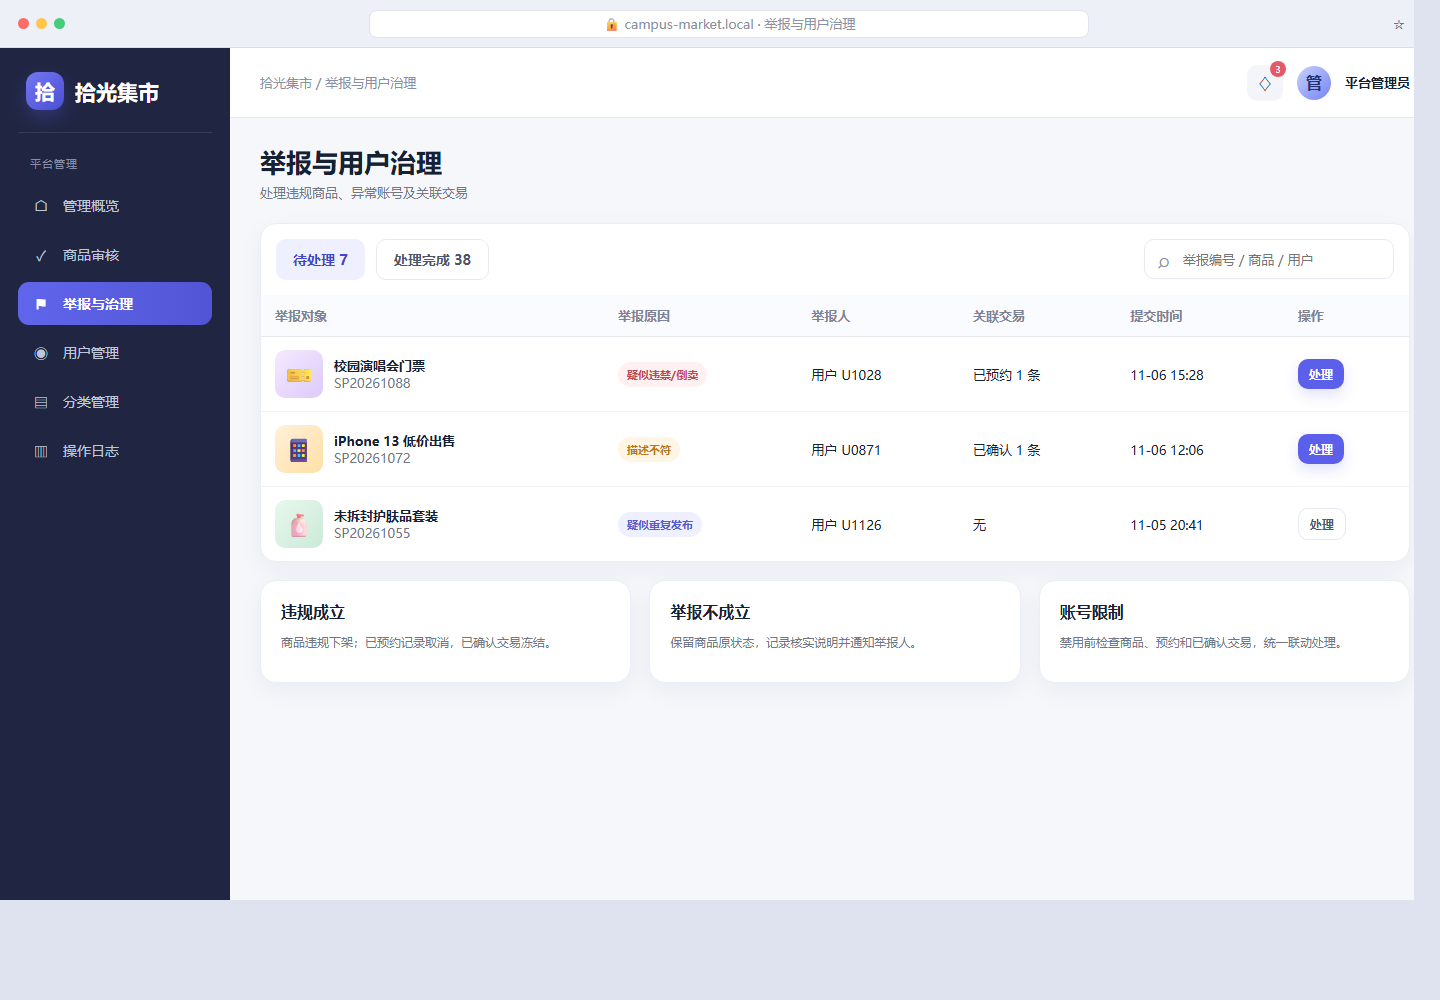
\includegraphics[width=\linewidth]{11_举报与用户治理.png}
\caption*{UI-11：举报与用户治理}
\end{minipage}\hfill
\begin{minipage}[t]{0.49\textwidth}\centering
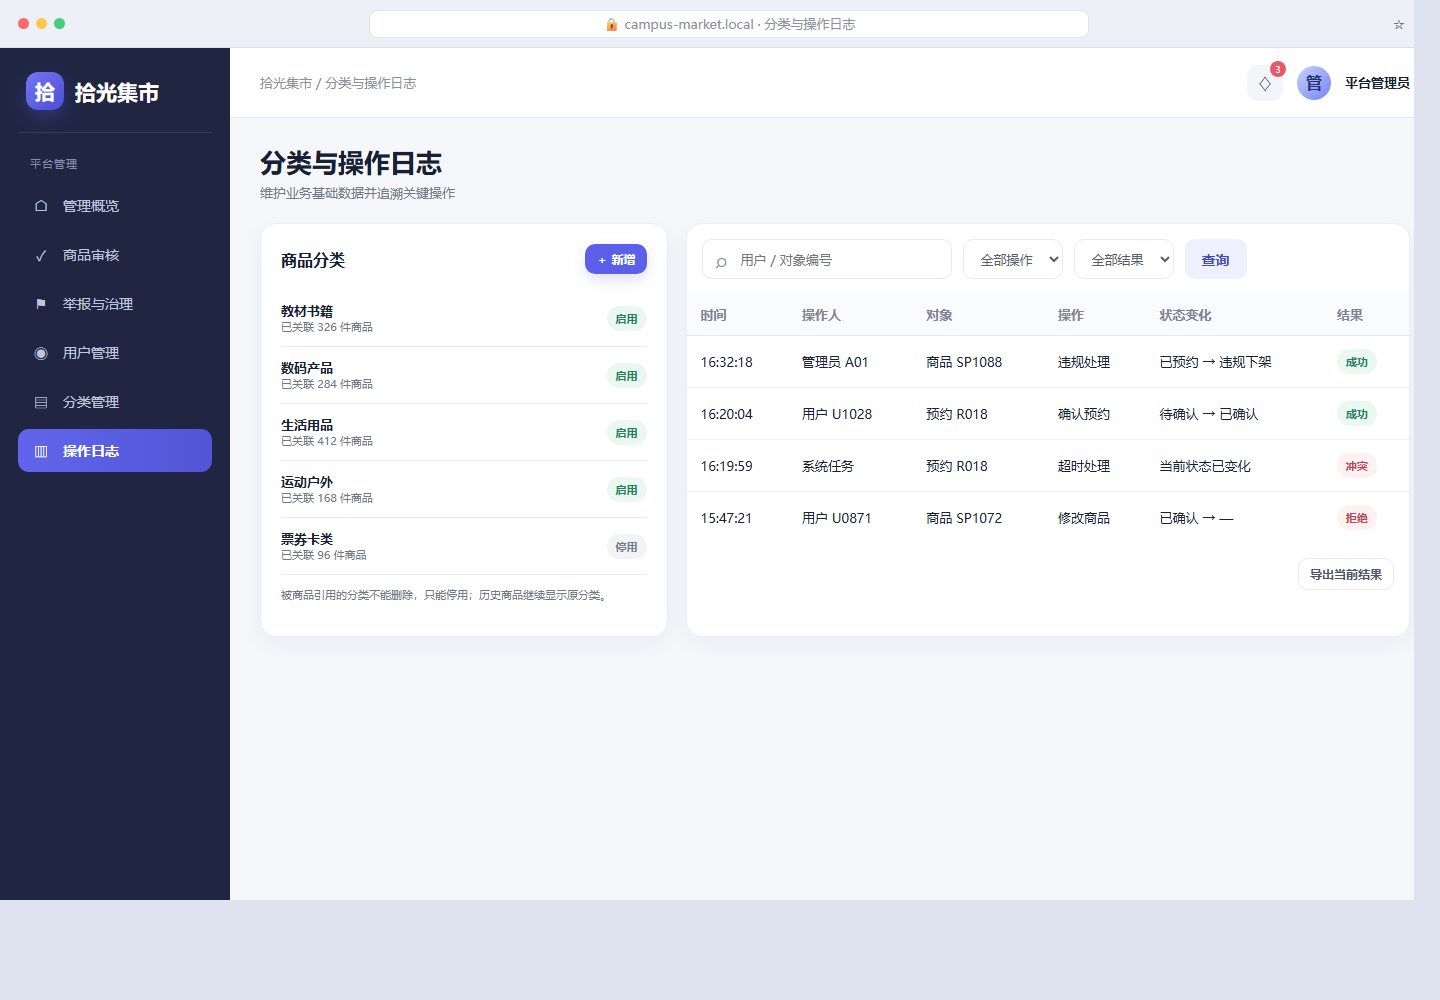
\includegraphics[width=\linewidth]{12_分类与操作日志.png}
\caption*{UI-12：分类与操作日志}
\end{minipage}
\caption{平台治理、分类和日志}
\end{figure}

举报列表同时显示商品、原因和关联交易状态，提醒管理员处理违规时同步预约或冻结交易。分类管理遵守“被引用后不能物理删除”的规则。日志页面展示成功、拒绝和状态冲突结果，使并发行为也能被追踪。

\section{AI辅助设计过程与人工判断}

\subsection{使用场景一：从需求基线到架构初稿}

\textbf{输入与生成结果：}将实验一的 20 条需求、角色、状态和异常规则作为上下文，要求 AI 给出模块划分和 UML 组件图。初稿选择了前端、认证、用户、商品、审核、查询、预约、通知、日志和调度模块，并提出 MySQL、Redis 和对象存储三类基础设施。

\textbf{优点：}AI 能快速检查基本功能是否都进入架构，尤其没有遗漏实验一中的审核、举报、通知和日志模块；同时给出了模块间调用关系，适合作为讨论起点。

\textbf{问题与人工判断：}初稿容易把系统拆成微服务，或者默认加入消息队列等常见技术。结合课程项目规模和商品—预约一致性要求，本设计决定采用模块化单体，暂不引入分布式事务和独立消息中间件。Redis 只做幂等和缓存，最终状态仍由 MySQL 保证。

\subsection{使用场景二：生成 PlantUML 并检查业务语义}

\textbf{输入与生成结果：}让 AI 依据实验一状态规则生成类图、用例图、状态图、活动图和预约并发时序图的 PlantUML 源码，再使用 PlantUML 本地渲染。生成过程中实际发现时序图把并行片段的第二分支写成不被 PlantUML 接受的关键字，语法检查失败。

\textbf{优点：}代码化 UML 便于版本比较、重复渲染和批量检查；状态图和时序图能够暴露仅靠文字不容易发现的空白，例如取消申请中商品仍是已确认，以及超时任务和卖家确认可能竞争。

\textbf{问题与人工优化：}语法正确不代表设计正确。人工需要逐图对照需求编号，确认角色、允许转换和禁止转换没有被 AI 自行改变；还需要检查图的密度和线条交叉，决定哪些关系保留在主图、哪些放到文字说明。

\subsection{使用场景三：UI方案生成与视觉检查}

\textbf{输入与生成结果：}根据功能模块和角色生成统一视觉规范，并设计 12 个高保真页面。页面采用蓝紫主色、卡片式布局和统一状态标签，以本地 HTML/CSS 原型导出为 1440×1000 PNG。

\textbf{优点：}AI 能较快保持控件、颜色和间距一致，并把需求中的 24 小时超时、价格快照、重新审核、取消申请暂停完成等规则直接呈现在界面中。

\textbf{问题与人工优化：}AI 生成的页面容易只追求“看起来完整”，却忽略当前状态是否允许按钮出现。人工检查的重点不是装饰，而是每个页面的角色、状态和下一步是否与 UML 一致；还应检查文字对比度、危险操作层级、页面是否截断以及截图是否覆盖全部模块。

\subsection{使用场景四：报告整理与一致性校验}

AI 用于把图、界面和设计理由整理为报告结构，并生成图注和初步说明。人工需要核对每张图的名称、三类 UML 是否都覆盖、报告描述是否与图片一致、提交目录是否符合课程要求，以及 AI 使用过程是否真实保留了问题和修改，而不是只写“使用 AI 提高效率”。

\subsection{大模型能否让人只做检查校对}

可以设计一套高度自动化的辅助工作流：先冻结需求基线并建立需求—模块追踪表，再让模型生成 UML 源码和 UI 草稿；通过 PlantUML 语法检查、图片尺寸检查、文件清单检查和状态转换规则脚本自动发现明显问题；最后由人进行架构取舍、业务语义、隐私安全和视觉可用性评审。评审通过后，工具自动重新渲染、生成报告并创建 Git 标签。

但现阶段不适合让人只做形式化校对。模块边界、是否采用微服务、取消申请中的操作权限、违规时如何处理已确认交易等决策包含业务责任和风险，模型不能替甲方或设计者作最终决定。更合理的分工是让 AI 承担候选方案生成、格式转换和一致性初查，人负责需求来源、取舍理由、冲突解决和最终验收。

\section{阶段性结论}

本设计形成了 7 种 UML 图和 12 个主要 UI 页面，覆盖结构性、行为性和交互性建模要求。架构以模块化单体保证课程原型的可实现性，以商品版本、价格快照、条件状态更新、事务和幂等键落实实验一的数据一致性要求。UI 不仅展示功能入口，也展示状态、限制和异常处理。

当前版本作为 AI 辅助生成的设计初稿，下一步将以图的可读性、模块依赖和界面可用性为重点进行人工审查，并通过 Git 保留初稿和修改后的最终版本。

\end{document}
